\chapter{ANTLR}
ANTLR, Another Tool for Language Recognition, is a parser generator under a three clause BSD-license (\cite{antlrorg}).  It is a successor of PCCTS, sometimes called ANTLR v1, and the latest version is ANTLR v3. PCCTS was developed by Professor Terrence Parr of the University of San Francisco, now the primus motor behind ANTLR.

ANTLR generates recursive-decent recognizers that utilizes predicated LL(*) -- an extension to LL(k) that uses arbitrary lookahead to make decisions. LL parsers are often said to be more intuitive and easier for humans to read than e.g. LALR parsers. This is supported by the fact that most hand written parsers are LL parsers. ANTLR supports multiple target languages, including Java. There are generally three types of recognizers ANTLR can generate: lexers, parsers and tree parsers/walkers.

\section{LL(*)}
The LL(*) parsing strategy is a strategy unique to ANTLR, invented by Terrence Parr for ANTLR v3. It is much more powerful than traditional LL(k) parsing (\cite{definitiveAntlr}), because it is not limited to a finite amount of lookahead. It enhances the LL decision's predictive capabilities, but does not by means alter the recursive decent parsing strategy.  By automatically doing left-factoring LL(*) allows developers to write more natural and human readable grammar. If a grammar is specified as LL(k), LL(*) will degenerate into LL(k) for this grammar. A decision is LL(*) if a DFA exist that recognizes the decision's exact lookahead language and has the following (\cite{definitiveAntlr}):
\begin{itemize}
\item No unreachable states
\item No dangling states, i.e. states that cannot reach an accept state
\item At least one accept state for each alternative.
\end{itemize}
All alternatives have a lookahead language, and if the lookahead languages of the alternatives are disjoint, the decision is LL(*). Except for not having a finite lookahead, LL(*) differs from LL(k) with backtracking in that it is looking ahead with the DFA, and not the whole parser. A thorough description of LL(*) can be found in \cite{lookahead}.

\section{Grammar Specification}
\label{sect:antlr:grammarSpec}
The grammar is specified in a type of extended Backus-Naur form (EBNF), where the extension from BNF consists of the Kleene operators $?$, $ +$ and $\ast$, and the not-operator $\sim$.  In addition, ANTLR introduces some types of predicates, namely validating, hoisting and gated semantic predicates and syntactic predicates. Validating and disambiguating semantic predicates is on the form \verb!{sem. predicate}?!, gated semantic predicates is on the form \verb!{sem. predicate}?=>! and syntactic predicates is on the form \verb!(syn. pred.)=>!.

Member methods and variables of the parser can be placed in a \verb!@members{! members \verb!}! construct, and the corresponding \verb!@lexer::members{! members \verb!}! for the lexer. Actions specified in the target language can be inserted at appropriate places in the production rules wrapped in \verb!{! and \verb!}!. 

Lexer productions and token names start with a capital letter, and parser productions do not. It is possible, and even common, to specify both the lexer and parser grammar in one file, thus ANTLR will determine which productions that belong to the lexer and the parser respectively by looking at the case of the first letter in the name of the production rules. An example of ANTLR grammar can be seen in figure \ref{code:simpleGrammar}. This grammar will generate a parser that recognizes input such as "John is 37 years old".
\begin{figure}[h!]
\begin{verbatim}
NAME     : ( 'a'..'z' | 'A'..'Z')+;  
AGE      : ('1'..'9')? ('1'..'9'|'0');
sentence :  NAME ' is ' AGE  ' years old';
\end{verbatim}
\caption{ANTLR grammar example}
\label{code:simpleGrammar}
\end{figure}

\section{Lexer}
\label{sect:antlr:lexer}
Lexers generated by ANTLR is by default a class derived from \verb!Lexer! (in the \verb!org.antlr.runtime! package) with additional per lexer rule methods for matching incomming character data. The lexer depends upon a input module that implements the \verb!CharStream! (e.g. \verb!AntlrStringStream!) interface which defines the method \verb!public int LT(int k)!. This method returns the character in the input stream \verb!k! positions from the current position. The method \verb!public Token nextToken()! in the lexer will generate and return the next token found by the lexer in the character stream. An overview of this method can be seen in figure \ref{fig:nextToken}, where \verb!Lexer! is \verb!org.antlr.runtime.Lexer! and \verb!TestLexer! is the lexer generated by a fictional grammar \verb!Test!.

\begin{figure}[h]
\centering
\begin{tabular}{|l|l|l|} \hline
\textbf{Lexer} 				& \textbf{TestLexer} 			\\ \hline
\verb!CharStream input;!		& 					\\
					&					\\
\verb!nextToken(){!			&					\\
\verb!   token = NULL;!			&					\\
\verb!   pos = input.position!		&					\\
\verb!   text = NULL;!			&					\\
					& \verb!mTokens{!			\\ 
					& \verb!   _type = "predict type"!	\\
					& \verb!   input.updatePosition()!	\\
					& \verb!   this.type = _type;!		\\
					& \verb!}!				\\
\verb!   if(token == NULL){!		&					\\
\verb!     emit(){!			&					\\
\verb!        t=new Token(type, pos,! 	&					\\
\verb!            input.position, input);!&					\\ 
\verb!        t.setText(text)!		&					\\
\verb!        emit(t){!			&					\\
\verb!          token=t;}!		&					\\
\verb!     }!				&					\\
\verb!   }!				&					\\
\verb!   return token;!			&					\\
\verb!}!				&					\\ \hline
\end{tabular}
\caption{Pseudocode showing how the lexer generates tokens.}
\label{fig:nextToken}
\end{figure}
Unless explicitly defined the tokens will hold the text they have matched as \verb!input!, \verb!startPosition! and \verb!endPosition!. It is also worth noticing that \verb!token! is set to \verb!NULL! for each token request, and a token will only be generated by \verb!nextToken()! if \verb!token! still has the value \verb!NULL! after the generated part of the lexer has decided which token to match.

When the lexer is to predict which type of token it should return (\verb!"predict type"! in figure \ref{fig:nextToken}), it peeks into the input character stream as many positions ahead needed to disambiguate the alternatives and make a decision. However, for e.g. to easily be able to define keywords, some ambiguous alternatives are allowed. ANTLR will then choose between the alternatives following some simple rules:
\begin{itemize}
\item An explicit expressed character sequence is chosen before an implicit one.
\item A longer sequence is chosen before a shorter one.
\item A production declared before another is chosen first.
\end{itemize}
These rules are ranked, and ANTLR will only use as many of them needed to differanciate the alternatives. Syntactic and semantic predicates will also make an impact on the decisionmaking as seen later. Figure \ref{fig:grammarPrec} shows a grammar with ambiguous alternatives, a simplified version of the code generated can be seen in figure \ref{fig:codeGenerated} where you can see that the parser will choose \verb!AB! before \verb!A! (and thus \verb!A B!) and \verb!A! before \verb!ANY!.
\begin{figure}[h!]
\begin{verbatim}
A       : 'a';
B       : 'b';
AB      : 'ab';
ANY     : ('a'..'z')+;
\end{verbatim}
\caption{Grammar showing the precidence among rules}
\label{fig:grammarPrec}
\end{figure}

\begin{figure}[h!]
\begin{verbatim}
int alt = 4;
if(LA(1) == 'a')
      if(LA(2) == 'b')
            if(LA(3) >= 'a' && LA(3) <= 'z')
                  alt = 4;
            else
                  alt = 3;
      else
            alt = 1;
else if(LA(1) == 'b')
      if(LA(2) >= 'a' && LA(2) <= 'z')
            alt = 4;
      else
            alt = 2;
else if(LA(1) >= 'c' && LA(1) <= 'z')
      alt = 4;
else
      throw new NoViableAltException();
\end{verbatim}
\caption{Example of how ANTLR predicts token type.}
\label{fig:codeGenerated}
\end{figure}
Production rules declared with the keyword \verb!fragment! are rules that never will be implicitly considered as an alternative. Fragment rules depend upon being referenced by other rules, fragment or not.
If the lexer grammar is so big that it may not compile, ANTLR will substitute the inline DFAs with DFA objects for prediction. These objects are implemented as a set of transition tables. More about the DFA objects can be found in \cite{antlrCodeGen}.

\section{Parser}
\label{sect:antlr:parser}
The parser generated by ANTLR is very much analogous with the lexer. By default the parser will be derived from \verb!org.antlr.runtime.Parser!. In addition to the methods and variables inherited, the generated parser will contain one method per production rule in the parser grammar. The parser does not have one defined "starting rule", thus, each method will have a prediction algorithm similar to \verb!mTokens()! in the lexer. As with the lexer, the algorithm peeks into the input stream as many tokens forward needed to differentiate between the alternatives. The parser takes a object that implements \verb!TokenStream! as input, which again takes a \verb!TokenSource! (the base class of \verb!Lexer!) as input. \verb!TokenStream! contains a method \verb!LT(int k)!, and classes that implements this interface often include a method \verb!LA(int k)! which returns the type of the token returned by the other method. \verb!CommonTokenStream! is a simple implementation of \verb!TokenStream!, and recomended by the ANTLR Community (\cite{antlrorg}) in most cases. The first time the \verb!LA(int k)! method of \verb!CommonTokenStream! is called a buffer of tokens will be filled by calling the lexer's \verb!nextToken()! until it returns \verb!Token.EOF! -- the end of the input. This means that before the parser starts to try matching production rules, the lexer will be finished creating tokens. Parsing will commence by calling the method created for the top-most production in the grammar, which in the case of XQuery with full text extension is \verb!module()!.

\section{Generating an Abstract Syntax Tree}
\label{sect:antlr:ast}
By default, ANTLR will not generate an AST from the grammar specification.
However, by setting the \verb!output! option value to \verb!AST! in the grammar
header, ANTLR will generate a simple ``flat'' linked list consisting of all the
parsed tokens in the input. 

This flat AST can be structured by adding operators and rewrite rules to tell
ANTLR which tokens to use as root nodes in productions, and which to leave out
of the AST entirely. There are two primary operators for AST structuring, hat
(\^{}) and exclamation mark (!). These operators are postfixed to tokens to
promote them to root nodes and exclude them completely from the AST,
respectively. Figure \ref{code:astOperators} shows an example where the
paranthesis would be excluded from the AST, and the \verb!PLUS! token
would be promoted to root node with two \verb!expr! children.

\begin{figure}[h!]
\begin{verbatim}
sum : '('! expr PLUS^ expr ')'!;
\end{verbatim}
\caption{Simple AST structuring operators example}
\label{code:astOperators}
\end{figure}

Additionally, ANTLR provides the commodity of rewrite rules for tailoring AST
generation. Figure \ref{code:astRewriteRules} shows an example with a rule for
an if-statement. The ``arrow'' (->) marks the start of the rewrite rule. The hat
(\^{}) operator indicates that the first token in the list should be promoted to
root node. There is no need to use exclamation marks as simple omission will
leave unwanted tokens out of the AST. Also note that variables can be used
exactly like in grammar predicates.

\begin{figure}[h!]
\begin{verbatim}
if : 'if' expr 'then' s1=stmt 'else' s2=stmt 'endif'
     -> ^(IFEXPR expr $s1 $s2);
\end{verbatim}
\caption{Usage of simple AST rewrite rules}
\label{code:astRewriteRules}
\end{figure}

Sometimes it may be necessary to customize the AST by adding custom fields to
the nodes or performing certain operations on them not supported by the built-in
tree representations. This can be done by subclassing the BaseTree (or
CommonTree) classes as well as adding a custom tree adaptor class, and setting
the option \verb!ASTLabelType=MyCustomTreeClass! in the grammar file header.

\section{Semantic Predicates}
\label{sect:antlr:semantic_preds}
Even though LL(*) allows the parser to scan arbitrarily far forward for any symbol or sequence of symbols to distinguish alternatives, it still has some weaknesses - particularly so when it comes to recursive rules. Semantic predicates are boolean expressions evaluated during runtime used to specify the semantic validity of an alternative. Predicate in this case simply means conditional, and the term semantic implies you are talking about arbitrary boolean expressions rather than a syntactic condition.  As previously mentioned, ANTLR provides three types of semantic predicates:
\begin{itemize}
\item Disambiguating semantic predicates; which disambiguate syntactically identical alternatives.
\item Gated semantic predicates; which can dynamically turn on and off parts of the grammar.
\item Validating semantic predicates; which throw a recognition exception if the predicate fails.
\end{itemize}

\subsection{Validating Semantic Predicates}
\label{sect:antlr:val_semantic_preds}
If the expression being evaluated in a validating semantic predicate yields $false$, an exception is thrown, expressing that a semantic predicate has failed. These predicates are never included in the decision-making process. Validating semantic predicates can be very handy in cases where e.g. you want to restrain the possible values a tokens can have, or to check if a variable is being referenced before its declaration. An example of a validating semantic predicate can be seen in figure \ref{code:validateSemantic}.

\begin{figure}[h!]
\begin{verbatim}
expr    : N {Integer.parseInt($N.getText()).intValue() < 7}?
        | . . .
        ;
\end{verbatim}
\caption[Validating semantic predicate.]{A Validating semantic predicate checking if the number value of \texttt{N} is less than $7$.}
\label{code:validateSemantic}
\end{figure}
As can be seen from this example, a semantic predicate is simply any kind of boolean Java expression. This is a flexible solution, because the boolean expression can be wrapped in a method with boolean return type, which for example then can be placed inside a @members { } clause in the grammar file, or even as a static method in an external class. This makes it possible to add complex grammar logic without
disturbing grammar brevity, if necessary.

\subsection{Disambiguating Semantic Predicates}
Disambiguating semantic predicates are hoisted into the prediction decisions of the LL(*) recognizer, but only if no decision can be made by syntax alone. There are generally two cases where these types of predicates are really useful: when a property of a token must dictate how the parser interprets it, and when a surrounding construct or some runtime information should alter how the parser matches the current construct. In most cases when a validating semantic predicate is applied, it can be transformed into a disambiguating semantic predicate. This will result in a syntax error instead of an exception if the predicate evaluates to $false$.

To fully resolve a non-determinism with disambiguating semantic predicates, all alternatives that contribute to the non-determinism will have to be covered, as seen in figure \ref{code:disambigSemantic}. The DFA generated in figure \ref{code:disambigSemantic} is illustrated in figure \ref{fig:dfaDisambiguate}.

\begin{figure}[h!]
\begin{verbatim}
expr      : {pred1}? A 
          | {pred2}? A
          ;
\end{verbatim}
\caption{Disambiguating semantic predicates.}
\label{code:disambigSemantic}
\end{figure}

\begin{figure}[!h]
  \centering
    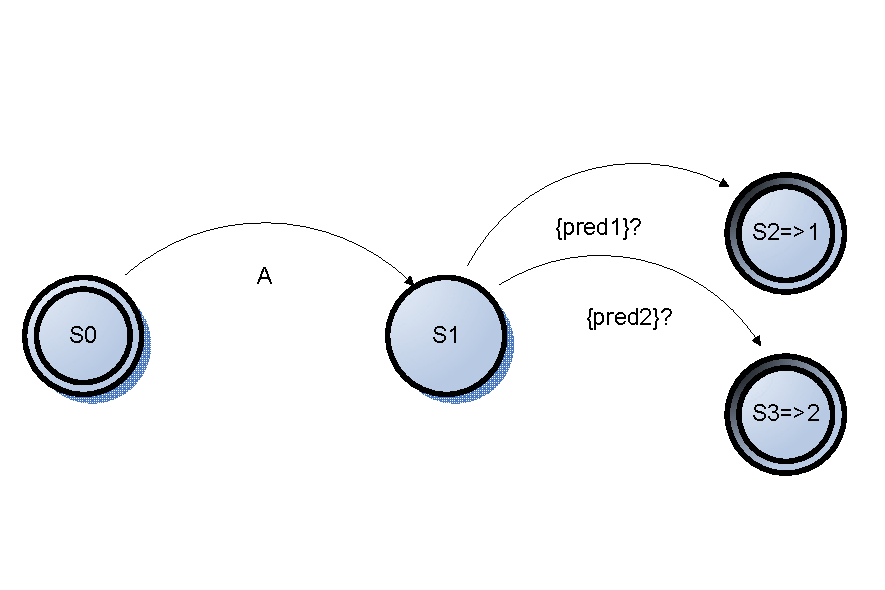
\includegraphics[scale=0.6]{img/disambigsemantic}
  \caption{The DFA of figure \ref{code:disambigSemantic}}
  \label{fig:dfaDisambiguate}
\end{figure}
As mentioned earlier, ANTLR hoists disambiguating semantic predicates into the state where the alternative prediction is made, which can be illustrated by the fact that the grammar inn figure \ref{code:disambigSemanticHoist} also yields the DFA shown in figure \ref{fig:dfaDisambiguate}. This includes only the predicates visible at the left edge of the production rule. 
\begin{figure}[h!]
\begin{verbatim}
expr      : a 
          | b
          ;
a         : {pred1}? A ;
b         : {pred2}? A;
\end{verbatim}
\caption{Hoisted disambiguating semantic predicates.}
\label{code:disambigSemanticHoist}
\end{figure}
Predicates implicitly specify precedence among the alternatives, where an earlier specified alternative has precedence over a later one. If both \verb!pred1! and \verb!pred2! would evaluate to true in figure \ref{code:disambigSemantic}., the first \verb!A! would be matched. In the case of only the first $n-1$ non-deterministic alternatives among $n$ are covered by a semantic predicate, the $n$th alternative would be covered with a \verb!{true}?! predicate. However, if this uncovered alternative was places first, it would be covered by a predicate that is the complement of the union of the following $n-1$ predicates.

\subsection{Gated Semantic Predicates}
\label{sect:antlr:gate_semantic_preds}
Gated semantic predicates are used when it is desirable to turn parts of a grammar on or off based on runtime information. The predicate will be hoisted into the decision even if the decision is deterministic by considering syntax alone. The difference between gated and disambiguating semantic predicates is that decisions use disambiguating semantic predicates only when syntax alone is insufficient to distinguish between alternatives. Figure \ref{code:gatedSemantic} shows an example of a gated semantic predicate, the resulting DFA is illustrated in figure \ref{fig:dfaGated}, showing how the predicate is hoisted even with no syntactic ambiguity.

\begin{figure}[h!]
\begin{verbatim}
expr      : a 
          | b
          ; 
a         : A;
b         : {pred}?=>B;
\end{verbatim}
\caption{Gated semantic predicate.}
\label{code:gatedSemantic}
\end{figure}

\begin{figure}[!h]
  \centering
    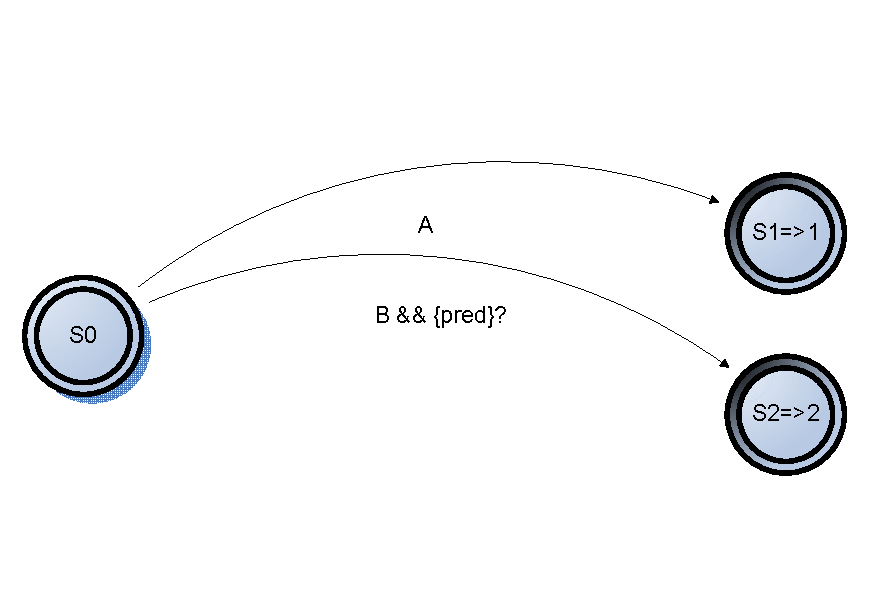
\includegraphics[scale=0.6]{img/gatedsemantic}
  \caption{The DFA of figure \ref{code:gatedSemantic}}
  \label{fig:dfaGated}
\end{figure}

\section{Syntactic Predicates}
\label{sect:antlr:syntacticPredicate}
Syntactic predicates are similar to semantic predicates except that they specify the syntactic validity of applying an alternative rather than the semantic validity. As with the semantic predicates their syntactic counterparts alter the parse based upon information available at runtime, but the only information the syntactic predicates use are future input symbols.  Both syntactic predicates and LL(*) support arbitrary lookahead, but whereas LL(*) uses a DFA to examine the future input symbols, the predicates use a pushdown machine, making them capable of recognizing more complicated structures in the lookahead than DFAs. Syntactic predicates are especially useful to specify the precedence between to ambiguous alternatives, or when LL(*) cannot handle the grammar the way you would like to write it.

When used to disambiguate between alternatives, ANTLR will try the alternatives in order. The alternative whose predicate is the first to return true, is the one chosen ("if it looks like A, it is A"). In its simplest form, syntactic predicates can be used to look ahead an arbitrarily number of symbols, to check if they match the symbols specified in the predicate. In a case like this ANTLR rewrites the predicate to a gated semantic predicate, an example of this is the grammar in figure \ref{code:syntactic} being translated to the equivalent grammar of figure \ref{code:translatedSyntactic}.

\begin{figure}[h!]
\begin{verbatim}
expr      : (A)=> A 
          | B
          ; 
\end{verbatim}
\caption{Syntactic predicate.}
\label{code:syntactic}
\end{figure}
\begin{figure}[h!]
\begin{verbatim}
expr      : {input.LA(1)==A}?=>A 
          | B
          ; 
\end{verbatim}
\caption{Translated syntactic predicate}
\label{code:translatedSyntactic}
\end{figure}

In more complex cases, syntactic predicates are implemented as disambiguating semantic predicates that invoke parser backtracking methods. These methods compare the input stream with the symbols specified in the predicate. If the stream and the symbols match, the method returns true, and the input stream is rolled back to the place where the comparing started. Such a case is exemplified by figure \ref{code:complexSyntactic}, where with an input such as "((a))" ANTLR will try the second alternative, succeed, backtrack, before telling the parser to choose this alternative.
\begin{figure}[h!]
\begin{verbatim}
expr      : (simple)=> simple ';'
          | (recur)=> recur ';'  
          | simple '!'
          ;
simple    : '(' ID ')';
recur     : '(' recur ')'
          | ID
          ;
ID        : ('a'..'z')+;
\end{verbatim}
\caption{A syntactic predicate which may backtrack}
\label{code:complexSyntactic}
\end{figure}

\section{Limitations in ANTLR}
\label{sect:parserconstructanddebug:limitations}
It is important to note, however, that ANTLR has limited support for unicode.
In this project this implies that our parser will not accept unicode characters
in the range from and above 0x10000. This will exclude the supplementary
multilingual plane (SMP) range of unicode characters, as well as the
supplementary ideographic plane (SIP) and the supplementary special-purpose
plane (SSP). These are seldomly used, but this is an important limitation
nonetheless. The Antlr developers have indicated that support for this unicode
range will be added in future versions of Antlr.

As a remedy for this situation it is possible to couple an external lexer with
ANTLR which will accept unicode characters in the above mentioned character
ranges. For the sake of simplicity this has not been further investigated nor
implemented in this project.
